\section{Planning}
In the previous sections, we focused on model-free algorithms (expect dynamic programming), where we \textbf{learned} policies or value 
functions by interacting with the environment, without any explicit model. Now, we shift to model-based settings, where we assume 
either that we can learn a model of the environment or are provided with one.\newline
\textbf{Planning} refers to any computational process that uses a model to produce or 
improve a policy for interacting with the modeled environment. We have already encountered 
planning in the context of value and policy iteration (Section \ref{dynammic programming}). 
In the following, we assume a model is available and explore various planning algorithms. 
(The next chapter will address how a model can potentially be learned.)

\subsection{Open-/Closed-Loop Planning}
In planning, we distinguish between open-loop and closed-loop planning.
In open-loop planning, the environment provides no feedback during execution. We are given 
an initial state and must immediately output a sequence of actions. For deterministic dynamics
this corresponds to solving an optimization problem to find the sequence of actions that maximizes the 
return :
$$a_1,\dots,a_T = \argmax\limits_{a_1,\dots,a_T} \underset{t=1}{\sum^T}r(s_t,a_t)\text{ s.t. } s_{t+1} = p(s_t,a_t)$$
In an environment with stochastic dynamics the optimization is stated as 
\begin{gather*}
    a_1,\dots,a_T = \argmax\limits_{a_1,\dots,a_T} \mathbb{E}\left[\underset{t=1}{\sum^T}r(s_t,a_t) \middle| a_1,\dots,a_T \right] 
    \quad s_{t+1} \sim p(s_{t+1}|a_t,s_t) \\
    \text{with } p(s_1,\dots,s_{T+1}|a_1,\dots,a_t) = p(s_1) \underset{t=1}{\prod^T p(s_{t+1}|a_t,s_t)} 
\end{gather*}
In open-loop planning, trajectories in stochastic environments are often suboptimal. Consider the analogy of taking an exam. Let’s say state 
$s_1$ represents the moment you receive the exam. The planned action sequence, in this case, corresponds to the answers you are going to give 
despite not knowing what the questions will be. Even if you're well-prepared, your answers are likely to be wrong, resulting in suboptimal 
outcomes since you can not look into the future. The fundamental problem is that open-loop plans cannot adapt to unexpected events or changes 
in the environment.We've already discussed open-loop methods like Random Shooting, Cross-Entropy Method (CEM), CMA-ES in section 
\ref{evo_strats}.\newline
In contrast, closed-loop planning allows the environment to provide feedback. In this 
setting, you’re given a state and asked to produce an action. After taking the action, the 
environment updates and returns the next state, continuing the cycle. This feedback loop 
enables more adaptive decision-making, as actions can be adjusted based on the state 
transitions and rewards observed during execution.
\begin{figure}[H]
    \centering
    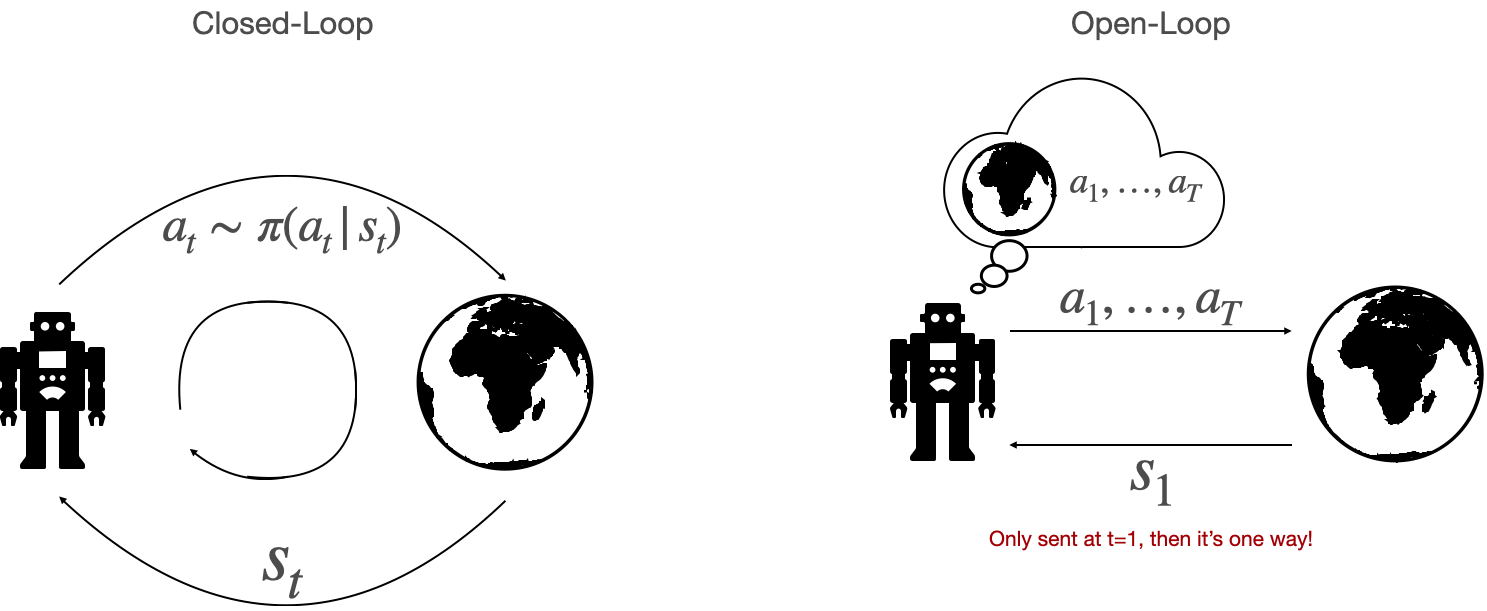
\includegraphics[width=0.9\linewidth]{images/closed_open_loop.png}
    \caption{Illustration of open- and closed-loop planning, inspired from ''CS 285: Lecture 10`` \cite{CS285,CS285LevineYoutube}}
    \label{fig:open_closed_loop}
\end{figure}

\subsection{Closed-Loop Planning in Discrete Domains - Monte-Carlo Tree Search}
For discrete domains, we have already explored dynamic programming approaches to derive 
policies given a model. However, in scenarios where the state space is large (e.g., Go, 
Chess, Atari, etc.), such methods become infeasible. An alternative is to use traditional 
tree search algorithms, but these also face limitations. For environments with huge 
branching factors, the search tree grows exponentially, making it computationally 
expensive.\newline
%Furthermore, tree search algorithms don't naturally handle stochastic transitions well.\newline
The approach we will be looking at next focuses on incrementally and asymmetrically building the 
search tree. Monte Carlo Tree Search (MCTS) addresses this by concentrating on the most 
promising moves and expanding the search tree through random sampling of the search space. 
MCTS consists of four main stages:
\begin{enumerate}
    \item \textbf{Selection:} start from root R and select successive child nodes until a leaf node L is reached. The root is the current game state and a leaf is any node from which no simulation (playout) has yet been initiated. The decision which child to take next is determined by the highest UCB-Score \ref{UCB}
    
    \item \textbf{Expansion:} unless the leaf L ends the game decisively (e.g. win/loss/draw) for either player, create one (or more) child nodes and choose node C from one of them. Child nodes are any valid moves from the game position defined by L. 
    
    \item \textbf{Simulation:} complete one random playout from node C. This step is sometimes also called playout or rollout. The rollout is typically performed with a default policy $\pi_\theta$. A playout may be as simple as choosing uniform random moves until the game is decided (for example in chess, the game is won, lost, or drawn).
    
    \item \textbf{Backpropagation} use the result of the playout to update information in the nodes on the path from C to R. For 1-0 (win-loss games), that means updating the win-loss counts of all the ancestor nodes. Note that the win count updates alternate between 0 or 1 (e.g. for black-white players) as you go up the tree.
\end{enumerate}
\begin{figure}[H]
    \centering
    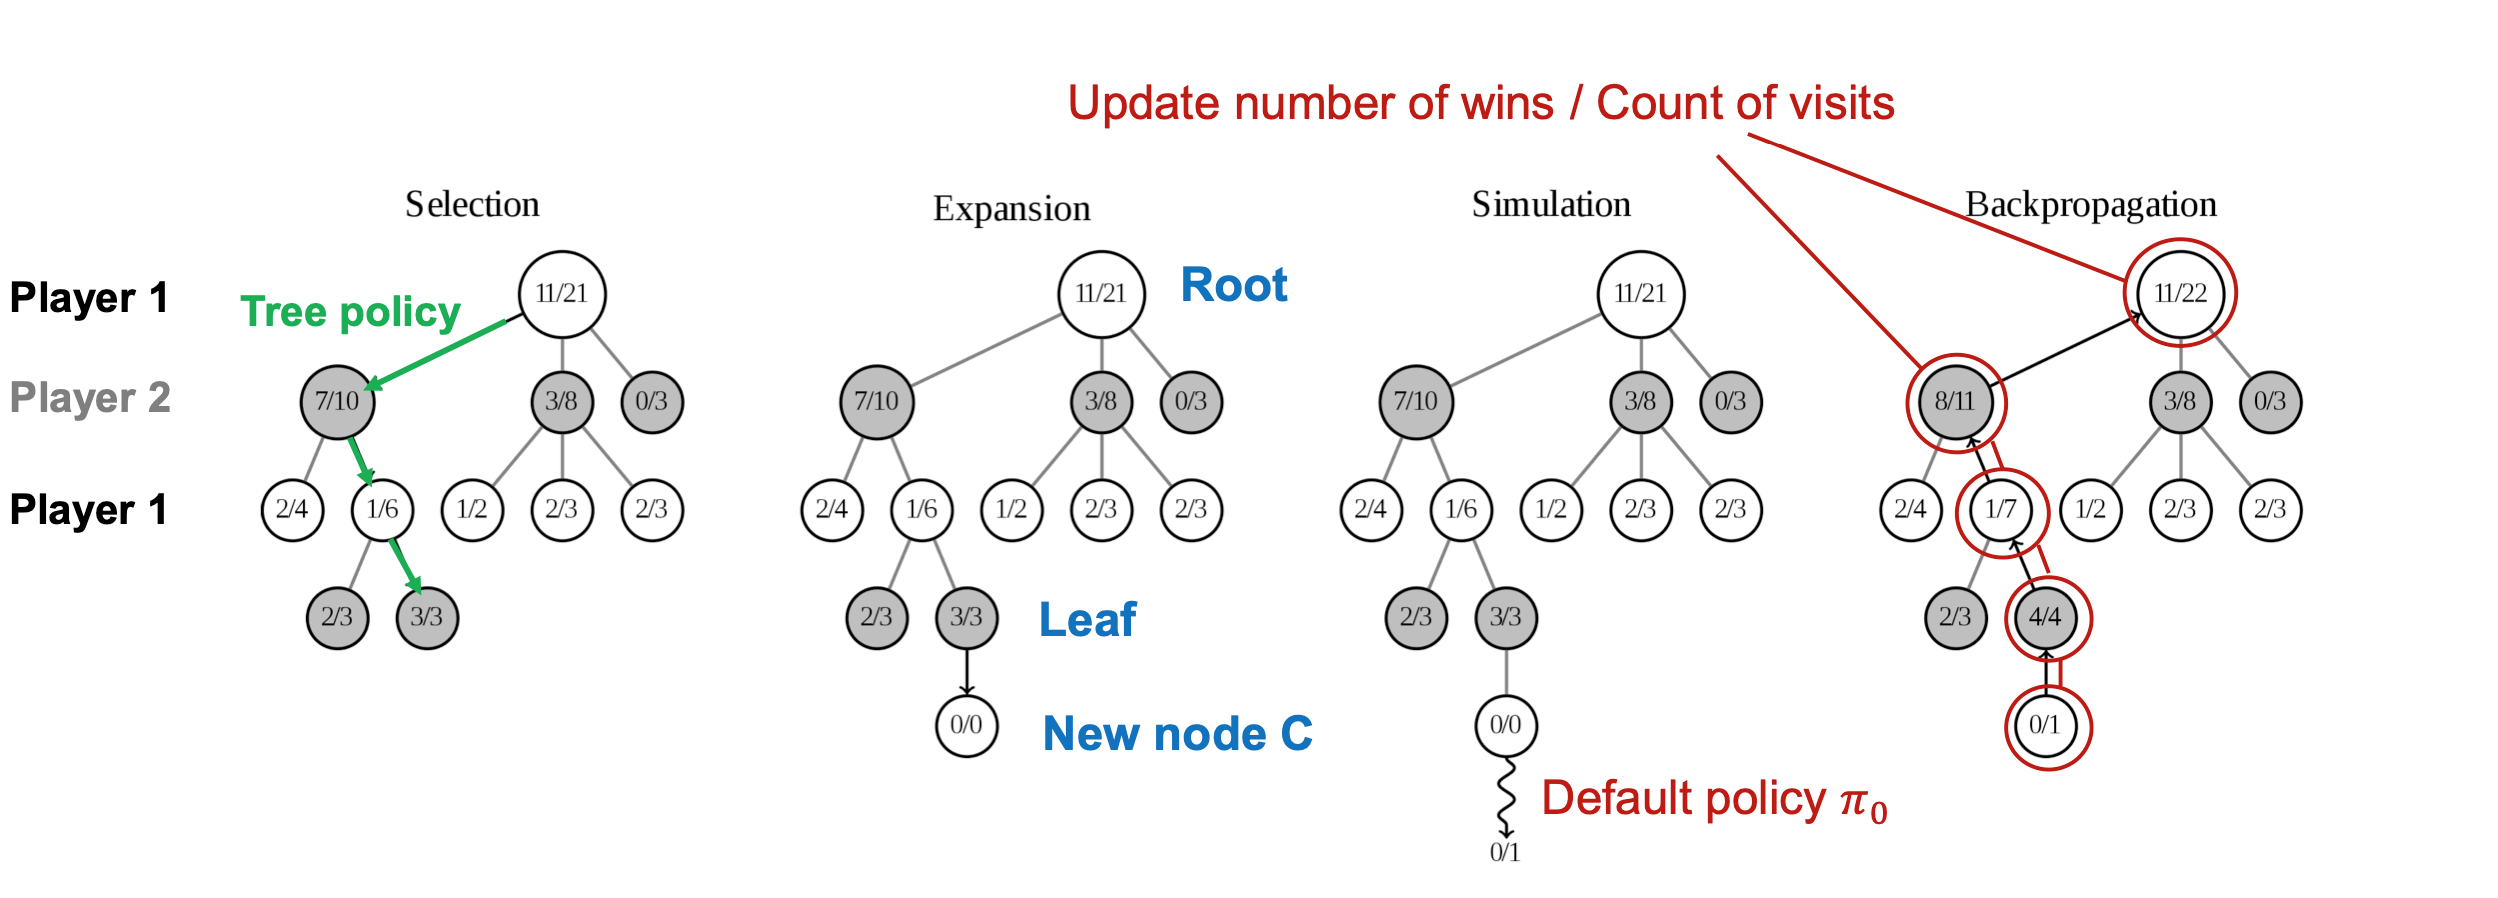
\includegraphics[width=\linewidth]{images/MCTS.png}
    \caption{The different phases of MCTS, image from KIT }
    \label{fig:MCTS}
\end{figure}
However, a major challenge arises when using Monte Carlo Tree Search (MCTS) in environments with continuous state and action spaces. In such 
cases, MCTS becomes significantly harder to apply effectively, as it's highly unlikely to encounter exactly the same states during planning.
This makes it difficult to build and reuse a meaningful search tree. To address this issue, we will explore an alternative method that is 
better suited for planning in continuous domains in the following chapter. But before we do that, we will first take a closer look at how 
MCTS has been used for planning in reinforcement learning.

\subsubsection{Alpha-Go and it successors}
\paragraph{AlphaGo} combined deep neural networks with Monte Carlo Tree Search (MCTS) and was trained using a combination of supervised 
learning from expert human games and reinforcement learning through self-play. It used separate networks to predict the best move (policy) 
and the likely winner (value).
\paragraph{AlphaGo Zero} is the successor to AlphaGo. AlphaGo Zero learned entirely from scratch, using only self-play without any human 
data. It also simplified the architecture by using a single neural network to predict both the policy and value, making it not only more 
efficient but also more powerful. This version surpassed the original AlphaGo despite having no prior knowledge of human strategies. 
\paragraph{AlphaZero}  generalized the approach from AlphaGo Zero. It used the same learning framework as AlphaGo Zero but was applied to 
different games, including Chess, Shogi, and Go. AlphaZero learned purely through self-play and used MCTS alongside a neural network, just 
like AlphaGo Zero, but it demonstrated that this method could be adapted to multiple environments with known rules.
\paragraph{MuZero} was the next major advancement. While AlphaZero still required a perfect simulator or full knowledge of the environment's 
rules, MuZero removed this assumption entirely. It learned not just the policy and value function, but also an internal model of the 
environment's dynamics—enabling planning without access to the real rules. Instead of learning to predict exact future states, MuZero learned 
a compact latent representation, from which it could plan and estimate rewards, values, and future outcomes.
\paragraph{AlphaTensor} was designed to discover new algorithms instead of learning to play games like Chess or Go. Specifically, it learns 
to find efficient matrix multiplication algorithms by framing the task as a single-player reinforcement learning problem.


A nice visualisation of how MCTS works and how it got used in AlphaZero/Go can be found \href{http://joshvarty.github.io/AlphaZero/}{here}.

\subsection{Resources}
Much of the content presented here is based on Sergey Levine’s CS 285: Lecture 10 \cite{CS285,CS285LevineYoutube}.
A helpful visualization of how Monte Carlo Tree Search (MCTS) works, particularly in the context of AlphaZero can be 
found on \cite{alphaZero}. For a technical breakdown of AlphaGo see the article \cite{alphaGo}, and for an overview 
of MuZero refer to DeepMind’s blog post \cite{muZero}.
